\documentclass{article} %basic LaTeX document type

%set capital Roman numeral section headings
%set capital Aramaic letters subsection headings
%set capital Arabic numbers subsubsection headings
\renewcommand\thesection{\Roman{section}.}
\renewcommand\thesubsection{\thesection\Alph{subsection}.}
\renewcommand\thesubsubsection{\thesubsection\arabic{subsubsection}.}

%set capital Roman numeral table numeration
\renewcommand*\thetable{\Roman{table}} 

%package needed for next lines
%makes section headings bold and upper case characters
%makes subsubsection headings in italics
\usepackage[explicit]{titlesec}
\titleformat{\section}{\bfseries}{\thesection}{1em}{\MakeUppercase{#1}}
\titleformat{\subsubsection}{\itshape}{\thesubsubsection}{1em}{#1}


%\linespread{2}       %option 1 for making text double-spaced
\usepackage{setspace} %option 2 for making text double-spaced
\doublespacing

%makes first paragraph of section indented (non-first are by default)
%set size of indentation (15pt is default)
\usepackage{indentfirst}
\setlength{\parindent}{25pt}

%set size of all margins
\usepackage[margin=1.3in]{geometry}
%can set margin sizes which are not the same in this way
%\usepackage[left=1in, top=1in, right=1in, bottom=1in]{geometry}

%package which returns number of last page (same as number of pages)
%package which counts the number of tables and/or figures
\usepackage{lastpage}
\usepackage[figure,table]{totalcount}

%enable `align' equation types
%enable `multirow' capability in tables
%enable figures
\usepackage{amsmath}
\usepackage{multirow}
\usepackage{graphicx}

%enables double spaced footnotes
\usepackage[]{footmisc}

%enables subfigures
%enables subfigure captions
%sets table caption formatting options to meet NSE requirements
%sets figure caption options to meet NSE requirements
\usepackage{caption}
\usepackage[labelformat=simple]{subcaption}
\captionsetup[table]{labelsep=newline,name=TABLE}
\captionsetup[figure]{name=Fig.,labelsep=period}

%sets labeling of footnotes
%double spacing of footnotes
\renewcommand{\thefootnote}{\alph{footnote}}
\renewcommand{\footnotelayout}{\doublespacing}

%enables proper labeling of subfigures
\renewcommand*\thesubfigure{(\alph{subfigure})}

%--------------
\usepackage{paralist}	
\usepackage{amssymb}
\usepackage{epsfig}
\usepackage[mathcal]{euscript}
\usepackage{setspace}
\usepackage{color}
\usepackage{array}
%\usepackage{subfigure}
\renewcommand{\ttdefault}{cmtt}
% The float package HAS to load before hyperref
\usepackage{float} % for psuedocode formatting
\usepackage{xspace}
\usepackage{mathrsfs}
\usepackage[pdftex]{hyperref}

%-------------
\DeclareMathOperator{\diag}{diag}
\DeclareMathOperator{\low}{lower}
\DeclareMathOperator{\upp}{upper}

\newcommand{\sa}{\shortrightarrow}
\newcommand{\bo}{\mathbf\Omega}
\newcommand{\vecr}{\textbf{r}}
\newcommand{\sn}{S$_\mathrm{N}$}
\newcommand{\pn}{P$_\mathrm{N}$}
\newcommand{\sigt}{\Sigma_t}
\newcommand{\sigs}{\Sigma_s}
\newcommand{\hl}{\mathcal{H}_L}
\newcommand{\maths}{\mathbb{S}^2}
\newcommand{\dl}{d_L}
\newcommand{\lij}{\langle L_i,L_j \rangle}
\newcommand{\kij}{\langle K_i,K_j \rangle}
\newcommand{\ve}[1]{\ensuremath{\mathbf{#1}}}
\newcommand{\Ye}[2]{\ensuremath{Y^e_{#1}(\bo_#2)}}
\newcommand{\Yo}[2]{\ensuremath{Y^o_{#1}(\bo_#2)}}
\newcommand{\Sigg}[1]{\ensuremath{\Sigma^{g'\sa g}_{\text{s},#1}}}
\newcommand{\even}{\ensuremath{\phi^g}}
\newcommand{\odd}{\ensuremath{\vartheta^g}}
\newcommand{\xhat}{\ensuremath{\hat{x}}}
\newcommand{\xbar}{\ensuremath{\bar{x}}}
\newcommand{\qhat}{\ensuremath{\hat{q}}}
\newcommand{\psihat}{\ensuremath{\hat{\psi}}}
\newcommand{\khat}{\ensuremath{\hat{K}}}
\newcommand{\Gij}[2]{\sum_{\ell=0}^L\frac{2\ell+1}{4\pi}P_{\ell}(\bo_#1\cdot\bo_#2)}
\newcommand{\Sij}[2]{\Sigma^{g'\rightarrow g}_{\text{s,L}}(\bo_#1\cdot\bo_#2)}
\newcommand{\Snij}[3]{\Sigma^{g'\rightarrow g}_{\text{s,#1}}(\bo_#2 \cdot \bo_#3)}
\newcommand{\Snz}[3]{\Sigma^{0\sa 0}_{\text{s,#1}}(\bo_#2 \cdot \bo_#3)}
\newcommand{\ldosig}[2]{\sum_{n=0}^N \frac{2n+1}{4\pi}\sigma_{s,n}^{g'\rightarrow g} P_n(\bo_#1\cdot\bo_#2)}
\newcommand{\fq}{\qquad\qquad\qquad\qquad}
\newcommand{\st}{\tilde{S}}
\newcommand{\E}[1]{$\times10^{#1}$}
\newcommand{\fwc}{\mbox{FW-CADIS}}

\begin{document}

%Define fields for \maketitle  (fields are \author, \date, \thanks, and \title)

\title{Assessment of the Lagrange Discrete Ordinates Equations for Monte Carlo Variance
Reduction Parameter Generation} %title of paper

\author{
\vspace{20mm}
%list of authors, with corresponding author marked by asterisk
\\Kelly L.\ Rowland,$^{\text{a}}$  Cory D.\ Ahrens,$^\text{b}$ Steven Hamilton,$^\text{c}$ 
\\and R.N.\ Slaybaugh$^{\text{a},\ast}$\\[4pt] 
%affiliations of authors
\textit{$^a$University of California, Berkeley, Nuclear Engineering Department}\\[-10pt]
\textit{4173 Etcheverry Hall, Berkeley, CA 94720, USA} \\[-5pt]
\textit{$^b$X Theoretical Design Division, Primary Physics Group}\\[-10pt]
\textit{Los Alamos National Laboratory, Los Alamos, NM 87545, USA}\\[-5pt]
\textit{$^c$Oak Ridge National Laboratory, Radiation Transport and Criticality Group} \\ [-10pt]
\textit{P.O. Box 2008, Oak Ridge, TN 37831-6170, USA} \\ [-2pt]
{$^\ast$slaybaugh@berkeley.edu}}       %address and email address for correspondence

%instead of returning the date, this repurposes the \maketitle command to print the number of pages, tables, and figures
\date{
\vspace{40mm}
Number of pages: \pageref{LastPage} \\  
Number of tables: \totaltables \\
Number of figures: \totalfigures \\}                                                                                           

\maketitle

\pagebreak

\begin{abstract}
{
abstract

Keywords: x; y; z
}
\end{abstract}

\pagebreak

%%---------------------------------------------------------------------------%%

\section{Introduction}
\label{sec:intro}

Radiation shielding is an important and interesting problem from various
perspectives. Simulation of shielding scenarios is critical for health physics
and nuclear security applications, but arriving at a solution for a given
response of interest (e.g., neutron flux at a given location) can be
computationally difficult in the context of
the magnitude of particle attenuation often seen in shielding problems.

The steady-state Boltzmann transport equation is typically solved using either 
deterministic methods or stochastic (Monte Carlo) methods. So-called ``hybrid''
methods aim to combine the favorable aspects of deterministic and Monte Carlo
methods to achieve better results. The CADIS (consistent adjoint driven
importance sampling) and \fwc\ (forward-weighted CADIS) methods are the current
state of the art in Monte Carlo variance reduction parameter generation.
Although hybrid methods are used to
significant effect in radiation shielding problems, they do not entirely
mitigate the negative aspects of the combined simulation types.

One particular area of study where hybrid methods tend to fall short is in
shielding problems with highly anisotropic particle movement and particle
streaming pathways. This is because the standard implementation of the CADIS
and \fwc\ methods is based on scalar particle flux rather than angular particle
flux. So, solutions from deterministic calculations exclude information about
how particles move toward a response of interest. For problems with strong
anisotropies in the particle flux, the importance map and biased source 
developed using the standard space/energy treatment may not represent the real
importance well enough to sufficiently improve efficiency in the Monte Carlo
calculation. 

This work aims to gauge the performance of Monte Carlo biasing parameters based
on scalar flux solutions from solving the Lagrange Discrete Ordinates (LDO)
equations. We will be employing the LDO equations' solutions in the standard
CADIS and \fwc\ methods to assess how well the LDO representation's unique
treatment of scattering and asymmetry in angle incorporate angular information
into the resultant scalar flux solutions and corresponding Monte Carlo biasing
parameters.

%%---------------------------------------------------------------------------%%
\section{Background}
\label{sec:background}

Here we begin by describing the CADIS (consistent adjoint driven importance 
sampling) and \fwc\ (forward-weighted consistent adjoint driven importance
sampling) methods, which are the current state
of the art of Monte Carlo variance reduction parameter generation. These are 
introduced first because this work 
employs solutions of the LDO equations in combination with the CADIS and \fwc\ 
methods via the ADVANTG software.

%%---------------------------------------------------------------------------%%
\subsection{CADIS and \fwc}

%%---------------------------------------------------------------------------%%
\subsubsection{CADIS}

The CADIS method was introduced by Wagner and Haghighat to automate Monte Carlo
variance reduction parameter generation \cite{cadis}. CADIS is based on the
source biasing and weight window techniques , does not depend heavily 
on user experience, and was implemented as described in Reference \cite{cadis}
in the MCNP \cite{mcnp} code. Most importantly, the result of using the CADIS
method is source biasing parameters and weight window target
values such that particles are born with the target weights.

The goal of most Monte Carlo transport problems is to calculate some response
(scalar flux, dose, etc.) at some location in phase-space. This can be posed as
solving the following integral equation:

\begin{equation}
R = \int_P \psi(P)\sigma_d(P)dP,
\label{eq:cadis_r1}
\end{equation}

\noindent where $R$ is the response of interest, $\psi$ is the neutron angular
flux, and $\sigma_d$ is some objective function in the phase-space
$(\vecr, E, \bo) \in P$. With the mathematical adjoint identity, it can be
shown that

\begin{equation}
R = \int_P \psi^{\dagger}(P)q(P)dP,
\label{eq:cadis_r2}
\end{equation}

\noindent where $\psi^{\dagger}$ and $q$ are the adjoint neutron angular flux
function and the particle source density, respectively. For a given problem
with a vacuum boundary condition, Equations \ref{eq:cadis_r1} and
\ref{eq:cadis_r2} are equivalent expressions for $R$. The adjoint neutron
angular flux function $\psi^{\dagger}$ has physical meaning as the expected
contribution to the response $R$ from a particle in phase-space $P$. In other
words, the adjoint flux function is significant because it represents the
importance of those source particles to the response of interest.

To calculate the response with the Monte Carlo method, the independent
variables are sampled from the probability density function (PDF) $q(P)$.
However, this may not be the best PDF from which to sample, so an alternative
PDF $\qhat(P)$ can be introduced into the integral:

\begin{equation}
R = \int_P \left[\frac{\psi^{\dagger}(P)q(P)}{\qhat(P)}\right]\qhat(P)dP,
\end{equation}

\noindent where $\qhat(P) \geq 0$ and the integral of $\qhat(P)$ over $P$ is 
normalized to unity. Then, the alternative PDF $\qhat(P)$ that will minimize
the variance of the response is given by

\begin{equation}
\qhat(P) = \frac{\psi^{\dagger}(P)q(P)}{\int_P\psi^{\dagger}(P)q(P)dP}.
\label{eq:qhat}
\end{equation}

Because the source variables are sampled from this new biased PDF, the
statistical weight of the source particles must be corrected such that

\begin{equation}
w(P)\qhat(P) = w_0q(P),
\label{eq:cadis_w1}
\end{equation}

\noindent where $w_0$ is the unbiased particle starting weight and is set equal
to 1. Substituting Equation \ref{eq:qhat} into Equation \ref{eq:cadis_w1} and
solving for $w(P)$ gives the following expression for the statistical weight of
the particles:

\begin{equation}
w(P) = \frac{\int_P\psi^{\dagger}(P)q(P)dP}{\psi^{\dagger}(P)}
= \frac{R}{\psi^{\dagger}(P)}.
\label{eq:cadis_w2}
\end{equation}

\noindent Equation \ref{eq:cadis_w2} demonstrates an inverse relationship
between this adjoint (importance) function and the statistical particle weight.
With this, reduced variance can be achieved when all source and transport
sampling is proportional to its importance. The source particles' energy and
position are sampled from the biased source distribution

\begin{equation}
\qhat(\vecr,E) = 
\frac{\phi^{\dagger}(\vecr,E)q(\vecr,E)}
{\int_V\int_E\phi^{\dagger}(\vecr,E)q(\vecr,E) dE\ d\vecr} 
= \frac{\phi^{\dagger}(\vecr,E)q(\vecr,E)}{R}.
\label{eq:cadis_sb}
\end{equation}

To bias particles undergoing the transport process, the weight window technique
is applied. Weight window lower bounds $w_{\ell}$ must be calculated such that
the statistical weights defined in Equation \ref{eq:cadis_w2} fall at the
center of the weight window intervals. The width of a given interval is denoted
by $c_u = w_u/w_{\ell}$, the ratio of upper and lower weight window values. The
weight window lower bounds are then given by

\begin{equation}
w_{\ell}(\vecr,E) = \frac{w}{\left(\frac{c_u +1}{2}\right)} 
= \frac{R}{\phi^{\dagger}(\vecr,E)}\frac{1}{\left(\frac{c_u +1}{2}\right)}.
\label{eq:cadis_tb}
\end{equation}

\noindent Using this definition, the weight window technique then performs
particle splitting and/or rouletting consistent with the statistical weight
given in Equation \ref{eq:cadis_w3}.

The key result of the foregoing discussion is that the statistical weights of
the source particles are within the bounds of the weight windows. In other
words, the source-biasing parameters and the weight window target values are
consistent. This circumvents the potential of particles being immediately split
or rouletted upon birth and avoids the resultant degradation in computational
efficiency. We refer the reader to \cite{cadis} for a complete discussion of
results and analysis of the initial implementation of the CADIS method. The
CADIS method is very effective for automated optimization of localized
detectors but falls short of efficiently optimizing distributed responses.
\fwc, discussed in the next section, was developed to address this issue.

%%---------------------------------------------------------------------------%%
\subsubsection{\fwc}

\fwc, is a variation on the CADIS method to increase the efficiency of Monte
Carlo calculations of distributions and responses at multiple localized
detectors \cite{fwcadis}.

For this global variance reduction method, a response with uniformly-low
statistical uncertainty across all phase-space is desired. One way to target
this for a given Monte Carlo simulation is to uniformly distribute the
particles throughout the system. Though this is not a physical response, it is
a proxy for the goal of obtaining uniform uncertainty. It also indicates the
possibility of developing an adjoint importance function that represents the
importance of particles to achieving the goal of uniform particle distribution.

With this new problem formulation, the problem of calculating particle density
is cast into the response formulation:

\begin{equation}
R = \int_{4\pi}\int_{V}\int_{E}\psi(\vecr,E,\bo)f(\vecr,E,\bo)dE\ dV\ d\bo,
\end{equation}

\noindent where $f(\vecr,E,\bo)$ is some function that converts angular
particle flux to Monte Carlo particle density. The Monte Carlo particle 
density can be estimated by

\begin{equation}
m(\vecr,E,\bo) = \frac{n(\vecr,E,\bo)}{\bar{w}(\vecr,E,\bo)} 
= \frac{\psi(\vecr,E,\bo)}{\bar{w}(\vecr,E,\bo)v(\vecr,E,\bo)}
\end{equation}

\noindent and the total Monte Carlo density can be estimated by

\begin{equation}
R = \int_{4\pi}\int_{V}\int_{E}\psi(\vecr,E,\bo)
\left[\frac{1}{\bar{w}(\vecr,E,\bo)v(\vecr,E,\bo)}\right]dV\ dE\ d\bo.
\label{eq:fwcadis_r}
\end{equation}

If the average particle weight is set proportional to the physical particle
density, then the Monte Carlo particle density should be approximately uniform
in phase-space:

\begin{equation}
R = \int_{4\pi}\int_{V}\int_{E}\psi(\vecr,E,\bo)
\left[\frac{1}{\psi(\vecr,E,\bo)}\right]dV\ dE\ d\bo.
\end{equation}

\noindent By then defining the adjoint source as the bracketed term in the
above equation,

\begin{equation}
q^{\dagger}(\vecr,E,\bo) = \frac{1}{\psi(\vecr,E,\bo)},
\end{equation}

\noindent we can calculate an adjoint importance function that represents the
importance of particles to achieving the desired objective of uniformly
distributed Monte Carlo particles. This should, in turn, correspond to
approximately uniform statistical uncertainties. The method physically 
orresponds to weighting the adjoint source with the inverse of the forward
flux; the adjoint source will be high where the forward flux is low and the
adjoint source will be low where the forward flux is high. With this method,
after the adjoint has been determined, the standard CADIS procedures are used
to calculate consistent source biasing parameters and weight windows.

%%---------------------------------------------------------------------------%%
\subsection{LDO Equations}

\begin{itemize}
\item{Developed by Ahrens}
\item{Inherently 3D}
\end{itemize}

%%---------------------------------------------------------------------------%%
\section{Results}
\label{sec:results}

\begin{itemize}
\item{Compared LDO equations' associated MC VR parameters with those from
      standard quadrature sets}
\item{Relatively coarse multigroup energy library}
\end{itemize}

%%---------------------------------------------------------------------------%%
\subsection{Steel Plate Embedded in Water}

The first test case we describe is an idealized geometry of a steel plate 
embedded in water; it is modeled after the scenario presented in Reference 
\cite{wilsonslaybaugh}. 
A diagram of the problem geometry is shown in Figure \ref{steelxz} and a list
of material properties used in the problem is given in Table \ref{steel-mat}.
In Figure \ref{steelxz}, the orange region contains the source material, the 
black region is composed of steel, the blue regions indicate water, and the 
white region is composed of air.

\begin{figure}[!htb]
\centering
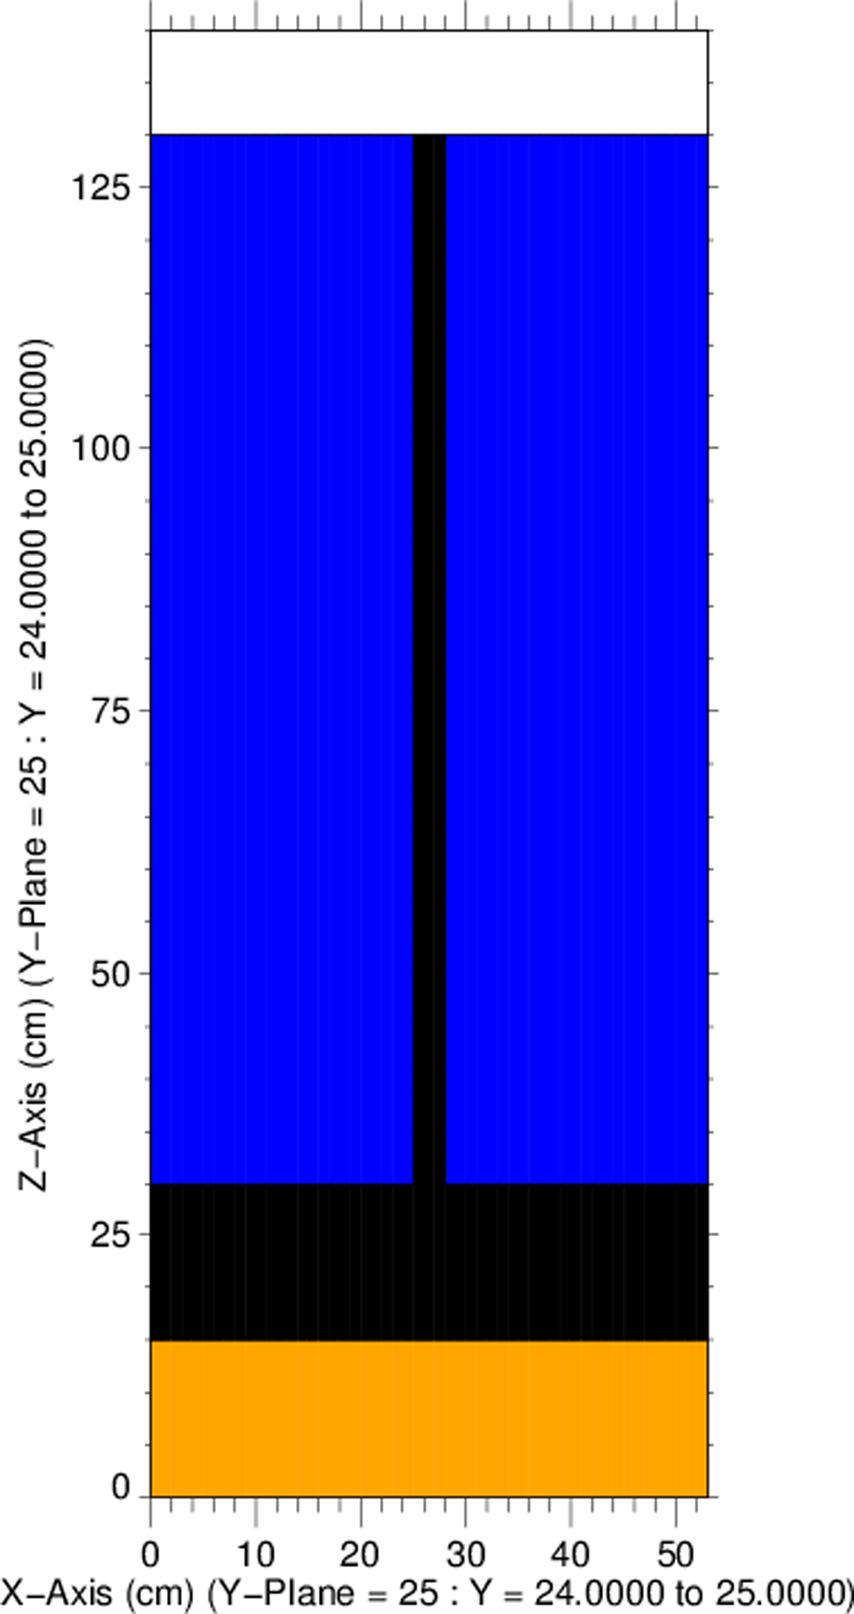
\includegraphics[width=0.4\textwidth]{img/steel-xz.png}
\caption{Steel plate in water geometry ($x-z$ slice through $y = 25$ cm) 
         \cite{wilsonslaybaugh}.}
\label{steelxz}
\end{figure}

The problem measurements are $53\times50\times140$ cm. The scenario is uniform 
in the $y$-direction and materials vary mainly in the $z$-direction. The source
region extends from 0 to 15 cm, the steel shield extends between 15 and 30 cm, 
the water and steel plate extend from 30 to 130 cm, and the air extends from 
130 to 140 cm. The steel plate is 3 cm wide and is centered at $x = 26.5$ cm. 
Vacuum boundary conditions were used at the problem boundaries.

A non-uniform Cartesian mesh was used for the spatial discretization in the 
deterministic calculations. In the $x$-direction, voxel width is 5 cm between
$x = 0$ cm and $x = 25$ cm, 0.5 cm between $x = 25$ cm and $x = 28$ cm, and 5 
cm between $x = 28$ cm and $x = 53$ cm. A uniform spacing of voxel width 1 cm 
was used in the $y$-direction. In the $z$-direction, the spatial cell width is
3 cm between $z = 0$ cm and $z = 30$ cm and 2 cm between $z = 30$ cm and 
$z = 140$ cm.

\begin{table}[!htb]
\centering
\caption{Materials and compositions in the steel plate in water scenario.}
\label{steel-mat}
\begin{tabular}{l|cc}
Material & \multicolumn{2}{c}{Isotopes (Atomic \%)} \\ \hline
\multirow{5}{*}{Source}   & U-235   & (0.000247) \\
                          & U-238   & (0.009287) \\
                          & Zr-nat. & (0.004009) \\
                          & H-1     & (0.037394) \\
                          & O-16    & (0.034927) \\ \hline
\multirow{4}{*}{Air}      & N-14    & (0.784431) \\
                          & O-16    & (0.210748) \\
                          & Ar-nat. & (0.004671) \\
                          & C-nat.  & (0.000150) \\ \hline
\multirow{2}{*}{Carbon Steel} & C-nat.  & (0.022831) \\
                              & Fe-nat. & (0.977169) \\ \hline
\multirow{2}{*}{Water}        & H-1     & (2)        \\
                              & O-16    & (1)        \\
\end{tabular}
\end{table}

The composition of the neutron source block is a homogenization of water,
zirconium, and uranium and was calculated based on the geometry and composition
of the Rowlands UO$_2$ pin cell benchmark specification \cite{pincell}. The
source is a U-235 fission 
spectrum that is uniformly distributed throughout the homogenized material. The
compositions of air, carbon steel, and water were taken from the Compendium of 
Material Composition Data for Radiation Transport Modeling \cite{pnnl}.

%%---------------------------------------------------------------------------%%
\subsection{Dog-Legged Void Neutron}

The next problem modeled is the dog-legged void neutron (DLVN) experimental 
benchmark, which was designed to measure neutron streaming in iron with air
voids. The model used in the following calculations was constructed from
References \cite{sw-dlvn,j-dlvn,dlvn1991}. The two materials used in the
problem are elemental iron and polyethylene. The polyethylene composition used
was C$_2$H$_4$. This is listed as ``polyethylene, non-borated'' and is material
248 in Reference \cite{pnnl}. 

\begin{figure}[!htb]
\centering
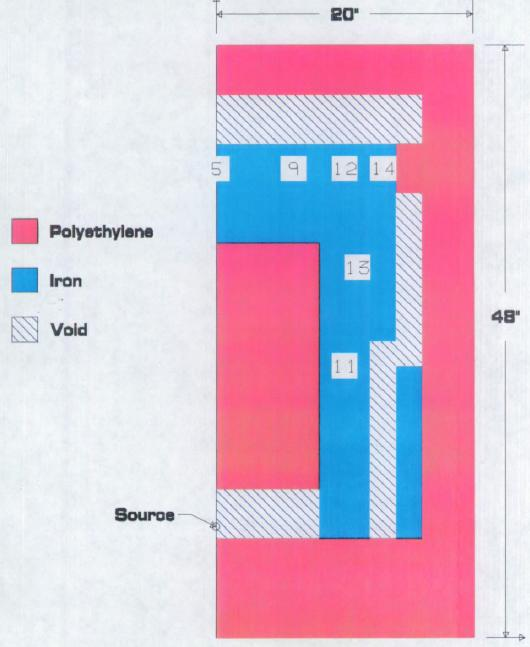
\includegraphics[width=0.5\textwidth]{img/dlvn.png}
\caption{Centerline cutaway of DLVN setup \cite{sw-dlvn}.}
\label{dlvn}
\end{figure}

The problem measurements are $40\times54\times48$ inches. A uniform spatial
mesh was imposed over the entire problem, with voxels measuring 1 inch per
side. The neutron source in this problem is a Cf-252 point source located at
the center of the $x-$ and $y-$directions and at $z = 9$ inches. This point
source was approximated as a small volumetric source in the tests in this
work.

The experimental configuration is symmetric about the $y-z$ plane at $x = 0$
and so is usually simulated with a reflecting boundary at $x = 0$ and vacuum
boundaries on all other sides of the configuration. For the tests in this work,
the use of reflecting boundary conditions was not available, so the model used 
was constructed to represent the entire experimental geometry configuration.
Vacuum boundary conditions were applied to the outside of the entire problem.

%---------------------------------------------------------------------------%%
\section{Conclusions}
\label{sec:conclusions}

\pagebreak
\section*{Acknowledgments}

This material is based upon work supported under an Integrated
University Program Graduate Fellowship as well as supported by the Department 
of Energy under Award Number(s) DE-NE0008661. This report was prepared as an
account of work sponsored by an agency of the United States Government.
Neither the United States Government nor any agency thereof, nor any of their
employees, makes any warranty, express or limited, or assumes any legal
liability or responsibility for the accuracy, completeness, or usefulness of
any information, apparatus, product, or process disclosed, or represents that
its use would not infringe privately owned rights. Reference herein to any 
specific commercial product, process, or service by trade name, trademark, 
manufacturer, or otherwise does not necessarily constitute or imply its 
endorsement, recommendation, or favoring by the United States Government or
any agency thereof. The views and opinions of authors expressed herein do not 
necessarily state or reflect those of the United States Government or any 
agency thereof. This research used the Savio computational cluster resource 
provided by the Berkeley Research Computing program at the University of 
California, Berkeley (supported by the UC Berkeley Chancellor, Vice Chancellor
for Research, and Chief Information Officer).

\pagebreak

\bibliographystyle{nse}
\bibliography{ldo-mc-vr}

\end{document}

